\subsection{Package sequenziatore.server.model}
\begin{figure}[H] \centering 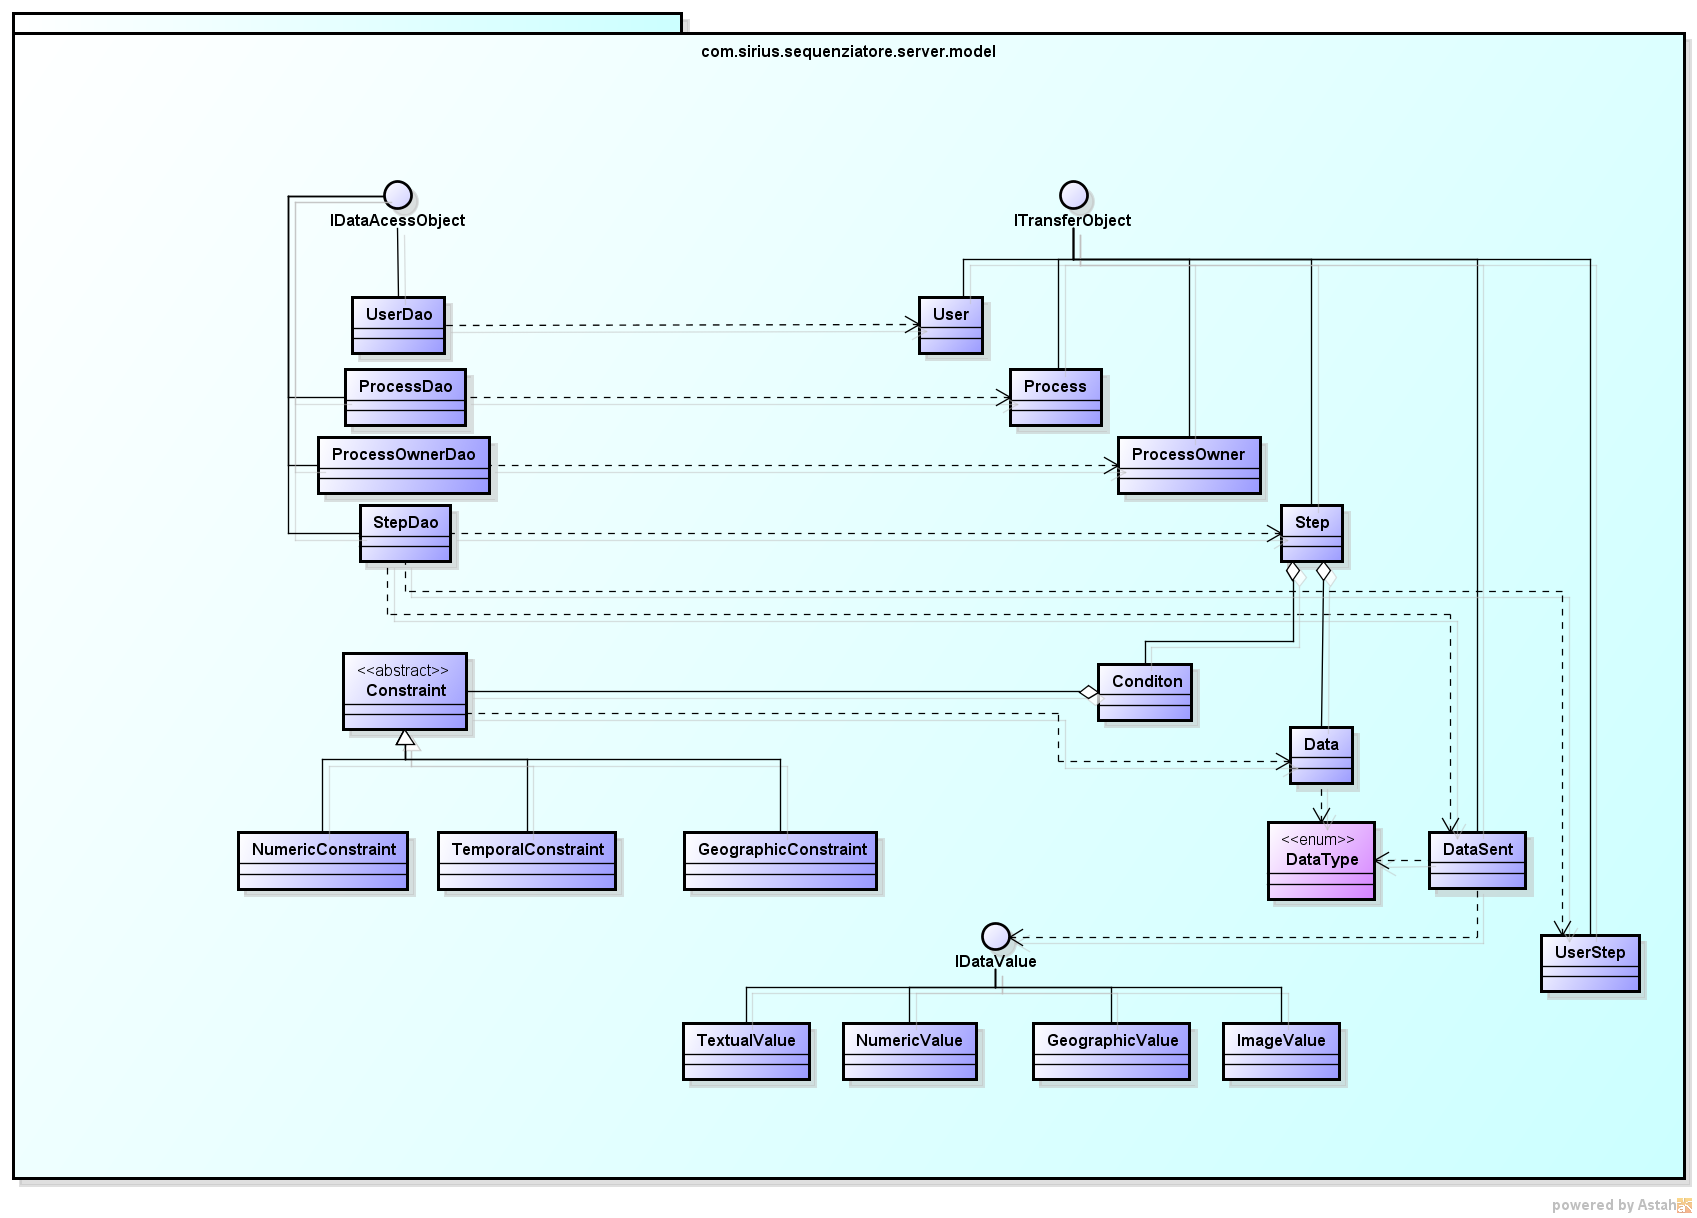
\includegraphics[width=%
\textwidth]
{./pack/ClassiServerSoloModel.png} \caption{Diagramma model server}
\end{figure}

\paragraph{IDataAcessObject}
\begin{itemize}
\item \textbf{Nome:} \texttt{IDataAcessObject};
\item \textbf{Package:} \texttt{\smodel{}};
\item \textbf{Descrizione:} Interfaccia che permette di gestire la comunicazione e l'interrogazione con il \textit{database}.
\end{itemize}

\paragraph{ITransferObject}
\begin{itemize}
\item \textbf{Nome:} \texttt{ITransferObject};
\item \textbf{Package:} \texttt{\smodel{}};
\item \textbf{Descrizione:} Interfaccia realizzata dai tipi che modellano i dati del \textit{database}.
\end{itemize}

\paragraph{UserDao}
\begin{itemize}
\item \textbf{Nome:} \texttt{UserDao};
\item \textbf{Package:} \texttt{\smodel{}};
\item \textbf{Descrizione:} Classe che si occupa delle interrogazioni del \textit{database} relative agli utenti del sistema.
\item \textbf{Relazione con altre componenti:} la classe implementa la seguente interfaccia:
		\begin{itemize}
			\item \smodel{}.IDataAcessObject.
		\end{itemize}
		La classe invoca i metodi della classe:
		\begin{itemize}
			\item \smodel{}.User.
		\end{itemize}
\end{itemize}

\paragraph{ProcessDao}
\begin{itemize}
\item \textbf{Nome:} \texttt{ProcessDao};
\item \textbf{Package:} \texttt{\smodel{}};
\item \textbf{Descrizione:} Classe che si occupa delle interrogazioni del \textit{database} relative ai processi.
\item \textbf{Relazione con altre componenti:} la classe implementa la seguente interfaccia:
		\begin{itemize}
			\item \smodel{}.IDataAcessObject.
		\end{itemize}
		La classe invoca i metodi della classe:
		\begin{itemize}
			\item \smodel{}.Process.
		\end{itemize}
\end{itemize}

\paragraph{ProcessOwnerDao}
\begin{itemize}
\item \textbf{Nome:} \texttt{ProcessOwnerDao};
\item \textbf{Package:} \texttt{\smodel{}};
\item \textbf{Descrizione:} Classe che si occupa delle interrogazioni del \textit{database} relative all'autenticazione del \textit{ProcessOwner}.
\item \textbf{Relazione con altre componenti:} la classe implementa la seguente interfaccia:
		\begin{itemize}
			\item \smodel{}.IDataAcessObject.
		\end{itemize}
		La classe invoca i metodi della classe:
		\begin{itemize}
			\item \smodel{}.ProcessOwner.
		\end{itemize}
\end{itemize}

\paragraph{StepDao}
\begin{itemize}
\item \textbf{Nome:} \texttt{StepDao};
\item \textbf{Package:} \texttt{\smodel{}};
\item \textbf{Descrizione:} Classe che si occupa delle interrogazioni del \textit{database} relative a tutte le operazioni sui passi dei processi.
\item \textbf{Relazione con altre componenti:} la classe implementa la seguente interfaccia:
		\begin{itemize}
			\item \smodel{}.IDataAcessObject.
		\end{itemize}
		La classe invoca i metodi della classe:
		\begin{itemize}
			\item \smodel{}.Step;
			\item \smodel{}.UserStep;
			\item \smodel{}.DataSent.
		\end{itemize}
\end{itemize}

\paragraph{User}
\begin{itemize}
\item \textbf{Nome:} \texttt{User};
\item \textbf{Package:} \texttt{\smodel{}};
\item \textbf{Descrizione:} Classe che modella gli utenti del sistema e che funge da interscambio dei dati di quest'ultimi con il \textit{database}.
\item \textbf{Relazione con altre componenti:} la classe implementa la seguente interfaccia:
		\begin{itemize}
			\item \smodel{}.ITransferObject.
		\end{itemize}
\end{itemize}

\paragraph{Process}
\begin{itemize}
\item \textbf{Nome:} \texttt{Process};
\item \textbf{Package:} \texttt{\smodel{}};
\item \textbf{Descrizione:} Classe che modella i processi del sistema e che funge da interscambio dei dati di quest'ultimi con il \textit{database}.
\item \textbf{Relazione con altre componenti:} la classe implementa la seguente interfaccia:
		\begin{itemize}
			\item \smodel{}.ITransferObject.
		\end{itemize}
\end{itemize}

\paragraph{ProcessOwner}
\begin{itemize}
\item \textbf{Nome:} \texttt{ProcessOwner};
\item \textbf{Package:} \texttt{\smodel{}};
\item \textbf{Descrizione:} Classe che modella il ProcessOwner e che funge da interscambio dei dati di quest'ultimo con il \textit{database}.
\item \textbf{Relazione con altre componenti:} la classe implementa la seguente interfaccia:
		\begin{itemize}
			\item \smodel{}.ITransferObject.
		\end{itemize}
\end{itemize}

\paragraph{Step}
\begin{itemize}
\item \textbf{Nome:} \texttt{Step};
\item \textbf{Package:} \texttt{\smodel{}};
\item \textbf{Descrizione:} Classe che modella i passi del sistema e che funge da interscambio dei dati di quest'ultimi con il \textit{database}.
\item \textbf{Relazione con altre componenti:} la classe implementa la seguente interfaccia:
		\begin{itemize}
			\item \smodel{}.ITransferObject.
		\end{itemize}
		La classe contiene istanze di:
		\begin{itemize}
			\item \smodel{}.Condition;
			\item \smodel{}.Data.
		\end{itemize}
\end{itemize}

\paragraph{DataSent}
\begin{itemize}
\item \textbf{Nome:} \texttt{DataSent};
\item \textbf{Package:} \texttt{\smodel{}};
\item \textbf{Descrizione:} Classe che modella i dati ricevuti dagli utenti che funge da interscambio  con il \textit{database}.
\item \textbf{Relazione con altre componenti:} la classe implementa la seguente interfaccia:
		\begin{itemize}
			\item \smodel{}.ITransferObject.
		\end{itemize}
				La classe invoca i metodi della classe:
		\begin{itemize}
			\item \smodel{}.IDataValue.
		\end{itemize}
\end{itemize}

\paragraph{UserStep}
\begin{itemize}
\item \textbf{Nome:} \texttt{UserStep};
\item \textbf{Package:} \texttt{\smodel{}};
\item \textbf{Descrizione:} Classe che modella i passi in corso e che funge da interscambio dei dati di quest'ultimi con il \textit{database}.
\item \textbf{Relazione con altre componenti:} la classe implementa la seguente interfaccia:
		\begin{itemize}
			\item \smodel{}.ITransferObject.
		\end{itemize}
\end{itemize}

\paragraph{Condition}
\begin{itemize}
\item \textbf{Nome:} \texttt{Condition};
\item \textbf{Package:} \texttt{\smodel{}};
\item \textbf{Descrizione:} Classe che modella le condizioni di avanzamento di un passo.
\item \textbf{Relazione con altre componenti:}La classe contiene istanze di:
		\begin{itemize}
			\item \smodel{}.Constraint;
		\end{itemize}
\end{itemize}

\paragraph{Data}
\begin{itemize}
\item \textbf{Nome:} \texttt{Data};
\item \textbf{Package:} \texttt{\smodel{}};
\item \textbf{Descrizione:} Classe che modella i campi dato richiesti.
\end{itemize}

\paragraph{Constraint}
\begin{itemize}
\item \textbf{Nome:} \texttt{Constraint};
\item \textbf{Package:} \texttt{\smodel{}};
\item \textbf{Descrizione:} Classe astratta che modella i vincoli.
\end{itemize}

\paragraph{NumericConstraint}
\begin{itemize}
\item \textbf{Nome:} \texttt{NumericConstraint};
\item \textbf{Package:} \texttt{\smodel{}};
\item \textbf{Descrizione:} Classe che modella i vincoli numerici..
\item \textbf{Relazione con altre componenti:} la classe estende la seguente classe:
		\begin{itemize}
			\item \smodel{}.Constraint.
		\end{itemize}
\end{itemize}

\paragraph{TemporalConstraint}
\begin{itemize}
\item \textbf{Nome:} \texttt{TemporalConstraint};
\item \textbf{Package:} \texttt{\smodel{}};
\item \textbf{Descrizione:} Classe che modella i vincoli temporali.
\item \textbf{Relazione con altre componenti:} la classe estende la seguente classe:
		\begin{itemize}
			\item \smodel{}.Constraint.
		\end{itemize}
\end{itemize}

\paragraph{GeographicConstraint}
\begin{itemize}
\item \textbf{Nome:} \texttt{GeographicConstraint};
\item \textbf{Package:} \texttt{\smodel{}};
\item \textbf{Descrizione:} Classe che modella i vincoli geografici.
\item \textbf{Relazione con altre componenti:} la classe estende la seguente classe:
		\begin{itemize}
			\item \smodel{}.Constraint.
		\end{itemize}
\end{itemize}

\paragraph{IDataAcessValue}
\begin{itemize}
\item \textbf{Nome:} \texttt{IDataValue};
\item \textbf{Package:} \texttt{\smodel{}};
\item \textbf{Descrizione:} Interfaccia che modella i valori dei dati ricevuti.
\end{itemize}

\paragraph{TextualValue}
\begin{itemize}
\item \textbf{Nome:} \texttt{TextualValue};
\item \textbf{Package:} \texttt{\smodel{}};
\item \textbf{Descrizione:} Classe che modella i valori dei dati testuali.
\item \textbf{Relazione con altre componenti:} la classe implementa la seguente interfaccia:
		\begin{itemize}
			\item \smodel{}.IDataValue.
		\end{itemize}
\end{itemize}

\paragraph{NumericValue}
\begin{itemize}
\item \textbf{Nome:} \texttt{NumericValue};
\item \textbf{Package:} \texttt{\smodel{}};
\item \textbf{Descrizione:} Classe che modella i valori dei dati numerici.
\item \textbf{Relazione con altre componenti:} la classe implementa la seguente interfaccia:
		\begin{itemize}
			\item \smodel{}.IDataValue.
		\end{itemize}
\end{itemize}

\paragraph{GeographicValue}
\begin{itemize}
\item \textbf{Nome:} \texttt{TextualValue};
\item \textbf{Package:} \texttt{\smodel{}};
\item \textbf{Descrizione:} Classe che modella i valori dei dati geografici.
\item \textbf{Relazione con altre componenti:} la classe implementa la seguente interfaccia:
		\begin{itemize}
			\item \smodel{}.IDataValue.
		\end{itemize}
\end{itemize}

\paragraph{ImageValue}
\begin{itemize}
\item \textbf{Nome:} \texttt{ImageValue};
\item \textbf{Package:} \texttt{\smodel{}};
\item \textbf{Descrizione:} Classe che modella i valori dei dati testuali.
\item \textbf{Relazione con altre componenti:} la classe implementa la seguente interfaccia:
		\begin{itemize}
			\item \smodel{}.IDataValue.
		\end{itemize}
\end{itemize}
